% !TeX program = pdflatex
% =============================================================================
% Zusatzdokument: Lorentzkraft Teil 1 -- Experiment 4: Fadenstrahlrohr
% UZH Praktikum I -- Sara Romer Urban, Kantonsschule im Lee, HS2026
% Klassen: 4fh (15.09.2026) + 4cdeg (18.09.2026) -- gemeinsames Material
%
% Herausgeloest aus arbeitsblatt6-lorentzkraft-teil1.tex (dieser Ordner), auf
% Wunsch als eigenstaendiges Dokument nur fuer diesen einen Versuch (eigene
% Station/eigenes Handout). Gehoert weiterhin zur selben Doppellektion wie
% Arbeitsblatt 6 -- Experimentnummerierung (Experiment 4) setzt dort direkt
% fort (1: Leiterschaukel, 2: Rollender Leiterstab, 3: Zwei parallele
% Leiter). KEINE eigene Arbeitsblatt-Nummer nach Sara Romers x/y-Schema
% (institutionen/UZH-Praktikum-I/CLAUDE.md), da dies kein neues,
% eigenstaendiges Arbeitsblatt-Thema ist, sondern ein aus Arbeitsblatt 6
% ausgegliederter Versuch derselben Doppellektion -- bei Bedarf umbenennen/
% umnummerieren, falls Sara Romer stattdessen eine fortlaufende
% Arbeitsblatt-Nummer dafuer moechte.
%
% Gegenueber der Fassung in Arbeitsblatt 6 zusaetzlich veraendert:
% - Der PhET/LEIFI-Simulationslink ("Simulation erkunden") ist entfernt --
%   der reale Versuch am Fadenstrahlrohr selbst deckt das bereits ab. Die
%   zugehoerige inhaltliche Frage (Wirkung von U_H, U_B, I_Spulen auf die
%   Bahn) bleibt aber erhalten, jetzt als Aufgabe "Die drei Messgroessen":
%   Herleitung/Begruendung anhand der Formel r=mv/(qB) statt Beobachtung
%   an der Simulation.
% - Neue Aufgabe "Geschwindigkeit der Elektronen" (E-Feld-Staerke im
%   Beschleunigungsfeld + Energieerhaltung fuer v) mit realistischen Werten
%   fuer Beschleunigungsspannung und Kathoden-Anoden-Abstand ergaenzt.
% - Hand-Konvention durchgehend auf technische Stromrichtung + rechte Hand
%   umgestellt (kein Wechsel auf die linke Hand mehr fuer Elektronen),
%   konsistent mit der ueberarbeiteten Lorentzkraft-Formelbox in
%   Arbeitsblatt 6.
%
% Quellen: lernziele.md, lorentzkraft-teil1-lektionsplan.tex (dieser Ordner),
% literatur/ (LEIFIphysik "Fadenstrahlrohr", "e/m an einer kleinen
% Fadenstrahlroehre"). Setzt die Lorentzkraft F=qvB (Arbeitsblatt 6) sowie
% die elektrische Feldstaerke E=U/d (Elektrizitaet: Ladung/E-Feld) als
% bekannt voraus.
%
% Bilder: siehe Bilder/*.png (Fadenstrahlrohr-Foto, Wehneltzylinder,
% Helmholtzspulen) und Bilder/*.jpg/*.pdf (Elektronenstrahl, Bahn-
% Illustration, allgemeine Kreisbahn einer positiven Ladung).
% =============================================================================
\documentclass[addpoints,11pt,a4paper]{exam}

\usepackage[T1]{fontenc}
\usepackage[utf8]{inputenc}
\usepackage[ngerman]{babel}
\usepackage{lmodern}
\usepackage[a4paper,margin=2.2cm,headheight=14pt]{geometry}
\usepackage{amsmath}
\usepackage{amssymb}
\usepackage{siunitx}
% Hausstil: zusammengesetzte Einheiten immer als echter Bruch (\frac), nicht
% als Inline-Schrägstrich oder \tfrac -- gilt global für jedes \si/\SI.
\sisetup{per-mode=fraction,fraction-command=\frac}
\usepackage{array,booktabs,tabularx,multirow}
\usepackage{enumitem}
\usepackage{xcolor}
\usepackage{colortbl}
\usepackage{tikz}
\usepackage{physics}
\usepackage{circuitikz}
\usepackage[most]{tcolorbox}
\usepackage{lastpage}
\usepackage{graphicx}
\usepackage{hyperref}

\usetikzlibrary{arrows.meta,calc,angles,quotes,decorations.markings,decorations.pathmorphing}

\usepackage{setspace}
\usepackage{needspace}
\setlength{\parindent}{0pt}
\setlength{\parskip}{0.6em}
\setstretch{1.08}
\setlist[itemize]{itemsep=0.4em}

% -----------------------------
% Farben (Corporate-Farbschema Physik KFR)
% -----------------------------
\definecolor{titleblue}{HTML}{183A6B}
\definecolor{accentblue}{HTML}{2E6F9E}
\definecolor{lightblue}{HTML}{EAF4FB}
\definecolor{verylightblue}{HTML}{F7FBFE}
\definecolor{lightgray}{HTML}{F4F6F8}
\definecolor{darkgray}{HTML}{4A4A4A}
\definecolor{accentorange}{HTML}{D9720C}
\definecolor{accentpurple}{HTML}{7B2D8E}
\definecolor{theorygreen}{HTML}{2E7D4F}
\definecolor{lighttheorygreen}{HTML}{EAF7EF}
\definecolor{groupteal}{HTML}{1B7F72}
\definecolor{lightgroupteal}{HTML}{E8F5F3}
\definecolor{lightorange}{HTML}{FCEEE0}
\definecolor{lightpurple}{HTML}{F3EAF7}

\hypersetup{
  colorlinks=true,
  urlcolor=accentblue,
  linkcolor=accentblue,
  pdftitle={Fadenstrahlrohr (Lorentzkraft, Teil 1)},
  pdfauthor={Loris Keller}
}

% -----------------------------
% Boxen (Praktikum I: Lernziele/Einleitung/Theorie/Aufgaben NICHT mehr farbig
% gerahmt -- nur Formel-, Hinweis- und Antwortbox bleiben Boxen, siehe
% institutionen/UZH-Praktikum-I/CLAUDE.md, Abschnitt "Boxen-Layout".)
% -----------------------------
\tcbset{before skip=10pt, after skip=10pt}
\newtcolorbox{titlebox}{
  enhanced,
  colback=titleblue,
  colframe=titleblue,
  boxrule=0pt,
  arc=3mm,
  left=3mm,right=3mm,top=3mm,bottom=3mm
}

\newenvironment{theoriebox}[1][Theorie]{%
  \par\addvspace{10pt}\noindent\textbf{#1}\par\smallskip\noindent
}{%
  \par\addvspace{10pt}
}

\newtcolorbox{taskbox}[1][]{
  enhanced, breakable,
  colback=white, colframe=white, boxrule=0pt,
  left=0mm,right=0mm,top=0mm,bottom=0mm,
  before skip=10pt, after skip=10pt,
  before upper={%
    \def\tmpboxtitle{#1}%
    \ifx\tmpboxtitle\empty\else\noindent\textbf{#1}\par\smallskip\fi
  }
}

\newtcolorbox{formelbox}[1][Formel]{
  enhanced,
  breakable,
  colback=lightpurple,
  colframe=accentpurple,
  title={#1},
  fonttitle=\bfseries,
  boxrule=0.9pt,
  arc=2mm,
  left=5mm,right=5mm,top=2mm,bottom=2mm
}

\newtcolorbox{answerbox}{
  breakable,
  colback=white,
  colframe=gray!55,
  boxrule=0.5pt,
  arc=1.5mm,
  left=2mm,right=2mm,top=2mm,bottom=2mm
}

% --- Lösungen ein-/ausblenden -----------------------------------------------
\noprintanswers
%\printanswers

\pointformat{}
\renewcommand{\solutiontitle}{\noindent\color{titleblue}\textbf{Lösung:}\enspace}

\pagestyle{headandfoot}
\cfoot{\textcolor{darkgray}{Seite \thepage\ von \pageref{LastPage}}}

\newcommand{\Kopfzeile}[4]{%
  \begin{titlebox}
    {\color{white}\sffamily\bfseries\Large #4}
  \end{titlebox}
  \vspace{0.5em}
  \noindent\textbf{Klasse:}~#1 \hfill \textbf{Datum:}~#2 \hfill \textbf{Thema:}~#3
    \hfill \textbf{Lehrperson:}~Loris Keller
  \vspace{0.8em}
  \lhead{\textcolor{darkgray}{#3}}
  \rhead{\textcolor{darkgray}{#4}}
}

\newlength{\antwortraumlen}
\newcommand{\Antwortraum}[1]{%
  \pgfmathsetlength{\antwortraumlen}{#1*2.5cm}%
  \begin{answerbox}
    \rule{0pt}{\antwortraumlen}%
  \end{answerbox}%
}

% Werte für Kopfzeile zentral setzen
\newcommand{\Klasse}{4fh / 4cdeg (SP4)}
\newcommand{\Datum}{15.09.2026 (4fh) / 18.09.2026 (4cdeg)}
\newcommand{\Thema}{Lorentzkraft (Teil 1): Fadenstrahlrohr}
\newcommand{\DokumentTitel}{Fadenstrahlrohr (Lorentzkraft, Teil 1)}

\begin{document}

\Kopfzeile{\Klasse}{\Datum}{\Thema}{\DokumentTitel}

\noindent Dieses Zusatzdokument gehört zur Doppellektion zur Lorentzkraft aus
Arbeitsblatt 6 und behandelt nur das vierte Experiment dieser Lektion, das
Fadenstrahlrohr. Die Lorentzkraft $F=qvB$ und die Drei-Finger-Regel mit der
technischen Stromrichtung setzen wir dabei als bekannt voraus.

% =============================================================================
% Experiment 4: Fadenstrahlrohr (Aufbau, ohne Kreisbahn vorwegzunehmen)
% =============================================================================
\begin{theoriebox}[Experiment 4 (Aufbau): Fadenstrahlrohr]
Die Lorentzkraft wirkt nicht nur auf Ladungen \emph{im} Leiter, sondern auch
auf eine \textbf{\emph{freie}} bewegte Ladung. Das \textbf{Fadenstrahlrohr}
macht genau das sichtbar. Die Elektronen selbst sind unsichtbar; ihre Bahn
wird erst durch das verdünnte Neongas im Glaskolben als leuchtende Spur
sichtbar gemacht, sobald sie mit den Gasteilchen zusammenstossen.
\begin{center}
  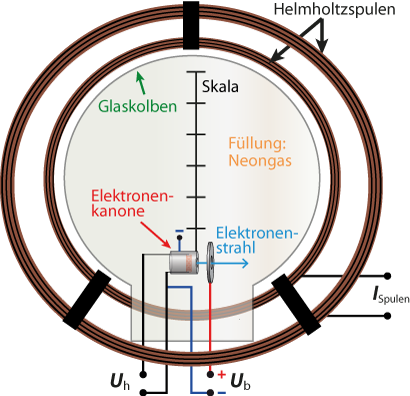
\includegraphics[width=6.5cm]{Bilder/fadenstrahlrohr.png}
\end{center}
{\scriptsize Aufbau: Elektronenkanone (Heizspannung $U_H$,
Beschleunigungsspannung $U_B$), Glaskolben mit Neongasfüllung und
Skala, Helmholtzspulen (Spulenstrom $I_\text{Spulen}$).}

\textbf{\emph{Wie entsteht das Licht, und woher kommt seine Farbe?}}
Trifft ein schnelles Elektron aus dem Strahl auf ein Neonatom im
Restgas, kann es einen Teil seiner Bewegungsenergie auf ein gebundenes
Elektron dieses Atoms übertragen. Dieses gebundene Elektron springt
dadurch auf ein höheres Energieniveau (\textbf{\emph{Anregung}}), ein
instabiler Zustand. Nach kurzer Zeit fällt es von selbst wieder auf ein
tieferes Niveau zurück (\textbf{\emph{Abregung}}) und gibt die dabei frei
werdende Energie als Lichtteilchen (Photon) ab.
\begin{center}
\begin{tikzpicture}[>=Latex,scale=0.85]
  % --- Teilbild 1: Anregung durch Stoss ---
  \begin{scope}
    \node[align=center,font=\bfseries\small] at (0,2.7) {1. Anregung durch Stoss};
    \draw[thick] (0,0) circle (1.0);
    \draw[thick] (0,0) circle (1.9);
    \filldraw[fill=gray!40] (0,0) circle (0.25) node[font=\scriptsize] {Ne};
    \node[font=\scriptsize] at (0,-1.25) {$E_1$ (Grundzustand)};
    \node[font=\scriptsize] at (0,-2.2) {$E_2$ (angeregt)};
    \filldraw[blue] (1.0,0) circle (0.07);
    \draw[thick,-{Latex[length=2.2mm]},blue,dashed] (1.0,0.15) to[bend left=45] (1.85,0.3);
    \node[blue,font=\scriptsize] at (1.65,0.85) {Anregung};
    \draw[thick,-{Latex[length=2.5mm]},red] (-3.1,1.6) -- (-1.05,0.35);
    \node[red,font=\scriptsize,align=center] at (-2.6,1.05) {schnelles $e^-$\\(Strahl)};
  \end{scope}
  % --- Teilbild 2: Abregung durch Lichtemission ---
  \begin{scope}[xshift=7.3cm]
    \node[align=center,font=\bfseries\small] at (0,2.7) {2. Abregung durch Lichtemission};
    \draw[thick] (0,0) circle (1.0);
    \draw[thick] (0,0) circle (1.9);
    \filldraw[fill=gray!40] (0,0) circle (0.25) node[font=\scriptsize] {Ne};
    \node[font=\scriptsize] at (0,-1.25) {$E_1$ (Grundzustand)};
    \node[font=\scriptsize] at (0,-2.2) {$E_2$ (angeregt)};
    \filldraw[blue] (1.85,0.3) circle (0.07);
    \draw[thick,-{Latex[length=2.2mm]},blue,dashed] (1.85,0.3) to[bend left=45] (1.0,0.15);
    \node[blue,font=\scriptsize] at (1.65,0.85) {Abregung};
    \draw[thick,orange,decorate,decoration={zigzag,amplitude=1.3pt,segment length=3.5pt}] (1.0,-0.3) -- (2.9,-0.3);
    \draw[thick,-{Latex[length=2.5mm]},orange] (2.9,-0.3) -- (3.25,-0.3);
    \node[orange,font=\scriptsize] at (2.05,-0.65) {Photon, $h\cdot f=E_2-E_1$};
  \end{scope}
\end{tikzpicture}
\end{center}
{\scriptsize Vereinfachtes Bohr-Modell eines Neonatoms: Stossanregung
durch ein Strahlelektron, gefolgt von Lichtemission beim Rücksprung auf
den Grundzustand.}

Jedes Element besitzt nur ganz bestimmte, diskrete Energieniveaus. Die
Photonenenergie entspricht deshalb immer genau der Differenz $\Delta
E=E_2-E_1=h\cdot f$ zwischen zwei solchen Niveaus, und diese Energie legt
über $f=\frac{c}{\lambda}$ die Wellenlänge (also die \textbf{Farbe})
des Lichts fest. Da das Fadenstrahlrohr mit Neongas gefüllt ist, leuchtet
die Elektronenspur deshalb in dem für Neon charakteristischen
Rötlich-Orange, wie man es auch von Neonröhrenreklamen kennt: Ein
anderes Füllgas würde eine andere Farbe ergeben, weil seine Atome andere
Energieniveaus besitzen.

\textbf{\emph{Die Elektronenkanone}} besteht aus drei Teilen: Die
\textbf{\emph{Glühkathode}} wird durch die Heizspannung $U_H$ erhitzt und
gibt dadurch freie Elektronen ab (glühelektrischer Effekt). Der
\textbf{\emph{Wehneltzylinder}} liegt leicht negativ und bündelt diese
Elektronen zu einem schmalen Strahl. Die \textbf{\emph{Anode}} liegt
positiv gegenüber der Kathode. Die dazwischen anliegende
Beschleunigungsspannung $U_B$ beschleunigt die Elektronen auf ihre
Geschwindigkeit $v$.
\begin{center}
  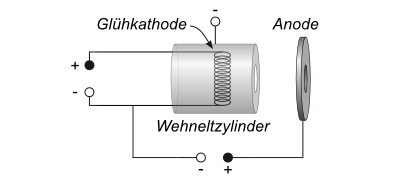
\includegraphics[width=7cm]{Bilder/Wehneltzylinder.png}
\end{center}
{\scriptsize Elektronenkanone: Glühkathode, Wehneltzylinder und Anode.}

\textbf{\emph{Die Helmholtzspulen}} sind zwei parallele, gleich
durchflossene Spulen im selben Abstand wie ihr Radius. Genau diese
Anordnung erzeugt dazwischen ein besonders \textbf{\emph{homogenes}}
Magnetfeld $B$. In dieses homogene Feld, senkrecht zu $v$, treten die
beschleunigten Elektronen ein.
\begin{center}
  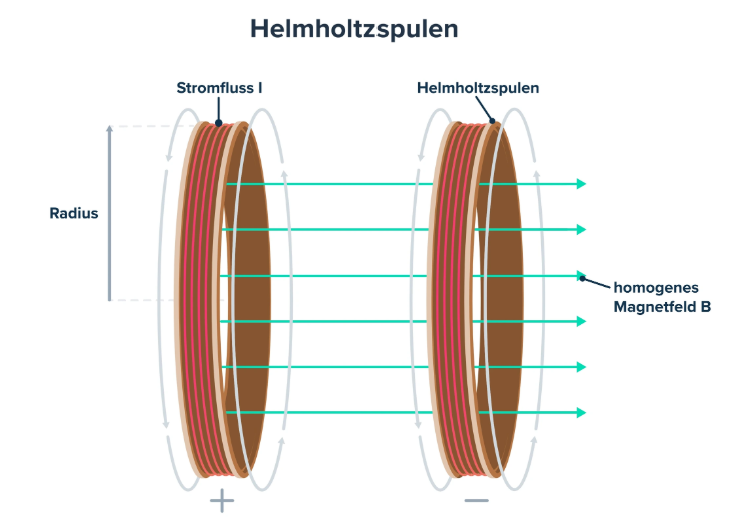
\includegraphics[width=8cm]{Bilder/Helmholtzspulen.png}
\end{center}
{\scriptsize Zwei Helmholtzspulen mit Stromfluss $I$ erzeugen zwischen
sich ein homogenes Magnetfeld $B$.}

Von oben betrachtet steht dieses Feld senkrecht zur Zeichenebene und zeigt
aus dem Blatt heraus (Symbol $\odot$). Was mit den Elektronen nach dem
Eintritt geschieht, untersuchen Sie in den folgenden Aufgaben.
\end{theoriebox}

% =============================================================================
% Aufgabe: Geschwindigkeit der Elektronen beim Eintritt ins Magnetfeld
% =============================================================================
\begin{questions}
\begin{taskbox}[Aufgabe: Geschwindigkeit der Elektronen]
\question Eine typische Elektronenkanone eines Fadenstrahlrohrs arbeitet
mit der Beschleunigungsspannung $U_B=\SI{300}{\volt}$; der Abstand
zwischen Glühkathode und Anode beträgt dabei realistischerweise nur etwa
$d=\SI{2}{\centi\meter}$.
\begin{parts}
  \part[2] Berechnen Sie die elektrische Feldstärke $E$ im
  Beschleunigungsfeld zwischen Kathode und Anode.
  \Antwortraum{2}
  \begin{solution}
  \[
    E = \frac{U_B}{d} = \frac{\SI{300}{\volt}}{\SI{0.02}{\meter}}
      = \SI{15000}{\volt\per\meter} = \SI{1.5e4}{\volt\per\meter}
  \]
  \end{solution}
  \part[4] Berechnen Sie mithilfe der Energieerhaltung die Geschwindigkeit
  $v$, mit der die Elektronen die Anode verlassen und ins Magnetfeld
  eintreten (Elektronenmasse $m_e=\SI{9.11e-31}{\kilo\gram}$,
  Elementarladung $e=\SI{1.6e-19}{\coulomb}$).
  \Antwortraum{4}
  \begin{solution}
  Die im elektrischen Feld verrichtete Beschleunigungsarbeit wird
  vollständig in kinetische Energie umgewandelt:
  \[
    e\cdot U_B = \frac{1}{2}\cdot m_e\cdot v^2
  \]
  Beide Seiten mit $2$ multiplizieren:
  \[
    2\cdot e\cdot U_B = m_e\cdot v^2
  \]
  Durch $m_e$ teilen:
  \[
    v^2 = \frac{2\cdot e\cdot U_B}{m_e}
  \]
  Wurzel ziehen:
  \[
    v = \sqrt{\frac{2\cdot e\cdot U_B}{m_e}}
  \]
  Einsetzen der Werte:
  \[
    v = \sqrt{\frac{2\cdot\SI{1.6e-19}{\coulomb}\cdot\SI{300}{\volt}}
      {\SI{9.11e-31}{\kilo\gram}}}
      \approx \SI{1.03e7}{\meter\per\second}
  \]
  Das sind rund $\SI{3.4}{\percent}$ der Lichtgeschwindigkeit: die
  klassische (nichtrelativistische) Rechnung mit $E_{\text{kin}}=\frac{1}{2}mv^2$
  ist damit noch gut gerechtfertigt.
  \end{solution}
\end{parts}
\end{taskbox}
\end{questions}

% =============================================================================
% POE: Fadenstrahlrohr (LZ6)
% =============================================================================
\begin{questions}
\begin{taskbox}[Predict-Observe-Explain: Fadenstrahlrohr]
\question Die Lehrperson führt jetzt das Fadenstrahlrohr vor.
\begin{parts}
  \part[2] \textbf{Predict.} Die Elektronen treten mit der Geschwindigkeit
  $v$ waagrecht in das Magnetfeld $B$ ein (Skizze unten). Die Lorentzkraft
  $F=qvB$ steht dabei (wie Sie in Arbeitsblatt 6 hergeleitet haben) immer
  senkrecht zu $v$. Überlegen Sie: Was bedeutet eine Kraft, die immer
  senkrecht zur momentanen Bewegungsrichtung steht, für die Bahn eines
  Teilchens? Zeichnen Sie die von Ihnen erwartete Elektronenbahn direkt
  ins Bild ein.
  \begin{center}
  \begin{tikzpicture}[>=Latex,scale=1.15]
    \begin{scope}
      \clip (0,0) circle (2.3);
      \foreach \x in {-2.1,-1.4,-0.7,0,0.7,1.4,2.1}{
        \foreach \y in {-2.1,-1.4,-0.7,0,0.7,1.4,2.1}{
          \node[font=\small,gray!65] at (\x,\y) {$\odot$};
        }
      }
    \end{scope}
    \draw[thick] (0,0) circle (2.3);
    % Elektronenkanone im UNTEREN Teil des Rohrs (wie im echten Aufbau),
    % Strahl tangential (waagrecht) nach rechts -- nicht radial auf den
    % Mittelpunkt gerichtet. Mit B aus dem Blatt heraus (⊙) und Strahl
    % nach rechts wirkt die Lorentzkraft auf das Elektron nach oben/innen.
    % Technische Stromrichtung (entgegengesetzt zu v, da Elektronen negativ
    % geladen sind) zeigt also nach links; rechte Hand: Daumen nach links,
    % Zeigefinger B aus dem Blatt heraus -> Mittelfinger nach oben -- von
    % unten gestartet zeigt "nach oben" ins Rohrinnere, also nach innen.
    \filldraw[black] (-0.3,-1.8) circle (0.08);
    \draw[thick,-{Latex[length=3mm]}] (-0.3,-1.8) -- (1.1,-1.8);
    \node[align=center] at (-0.3,-2.65) {\scriptsize Elektronenkanone};
    \node[align=left] at (0.45,-1.62) {\scriptsize $e^-$, $v$};
  \end{tikzpicture}
  \end{center}
  {\scriptsize Draufsicht auf das Rohr: $\odot$ = Magnetfeld $B$ der
  Helmholtzspulen (aus dem Blatt heraus). Die Elektronenkanone schiesst
  den Strahl tangential (waagrecht) nach rechts ins Feld.}
  \Antwortraum{2}
  \begin{solution}
  Eine Kraft, die immer senkrecht zur momentanen Geschwindigkeit steht und
  deren Betrag konstant bleibt (da $q$, $v$ und $B$ konstant sind), ändert
  nur die \emph{Richtung} von $v$, nie ihren \emph{Betrag}. Genau das ist
  die Bedingung für eine \textbf{Zentripetalkraft} aus der Mechanik. Zu
  erwarten ist deshalb eine \textbf{Kreisbahn}.
  \end{solution}
  \part[1] \textbf{Observe.} Beschreiben Sie kurz, was Sie am
  eingeschalteten Fadenstrahlrohr tatsächlich beobachten.
  \Antwortraum{1}
  \begin{solution}
  Die leuchtende Elektronenspur bildet tatsächlich eine geschlossene
  Kreisbahn.
  \end{solution}
  \part[3] \textbf{Explain.} Erklären Sie die beobachtete Kreisbahn
  physikalisch: Wirkt die Lorentzkraft hier als Zentripetalkraft?
  Bestimmen Sie ausserdem mit der Drei-Finger-Regel (\textbf{rechte
  Hand}) die Richtung, in die sich die Kreisbahn krümmt. Verwenden Sie
  dazu die \textbf{technische Stromrichtung}: Da Elektronen negativ
  geladen sind, zeigt der Daumen entgegen ihrer tatsächlichen
  Bewegungsrichtung $v$.
  \Antwortraum{3}
  \begin{solution}
  Ja: Die Lorentzkraft steht stets senkrecht zu $v$, ändert also nur die
  Bewegungsrichtung, nie den Geschwindigkeitsbetrag. Das entspricht genau
  der Definition der Zentripetalkraft, die die Elektronen auf ihrer
  Kreisbahn hält.

  Da Elektronen negativ geladen sind, verwenden Sie die technische
  Stromrichtung: Der Daumen zeigt entgegen der tatsächlichen
  Bewegungsrichtung $v$ der Elektronen. Mit der \textbf{rechten Hand}:
  Daumen entgegen $v$, Zeigefinger in Richtung $B$ (aus dem Blatt heraus,
  $\odot$). Der Mittelfinger zeigt dann anfangs zum Kreismittelpunkt der
  Bahn: Die Lorentzkraft lenkt die Elektronen entsprechend zur Seite
  ab. So sieht die Bahn tatsächlich aus, mit Schaltung, Radius $r$ und
  Zentripetalkraft $F_Z=F_L$ beschriftet:
  \begin{center}
  \begin{minipage}[t]{6.2cm}\centering
    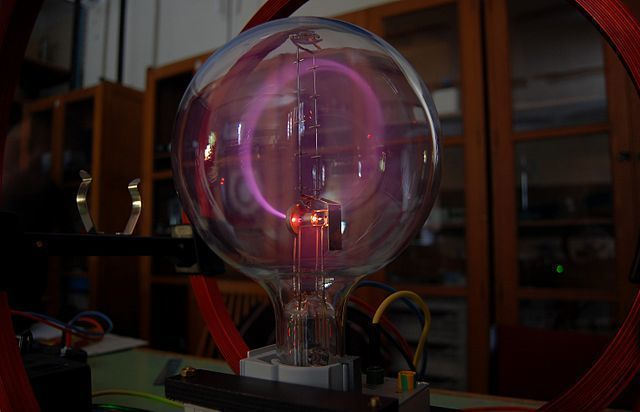
\includegraphics[width=6cm]{Bilder/beam-of-electrons.jpg}\\
    {\scriptsize Echtes Fadenstrahlrohr: die leuchtende Elektronenspur.}
  \end{minipage}\hfill
  \begin{minipage}[t]{6.5cm}\centering
    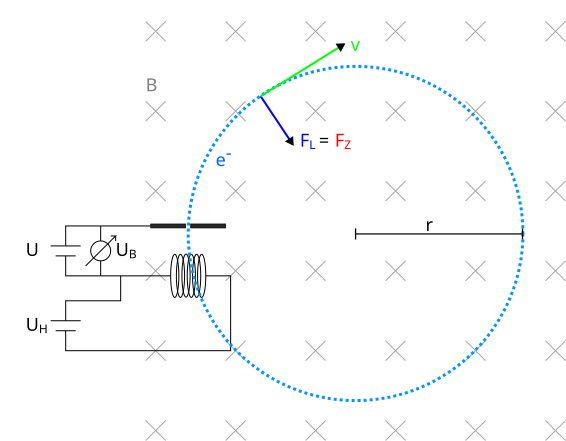
\includegraphics[width=6.2cm]{Bilder/Fadenstraglrohr_illustration.pdf}\\
    {\scriptsize $U$/$U_B$: Beschleunigungsspannung, $U_H$: Heizspannung,
    $r$: Bahnradius.}
  \end{minipage}
  \end{center}
  Dasselbe Prinzip gilt allgemein für jede frei bewegliche Ladung in einem
  homogenen Magnetfeld, nicht nur für Elektronen im Fadenstrahlrohr:
  \begin{center}
    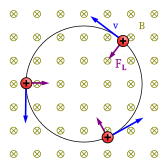
\includegraphics[width=5.5cm]{Bilder/proton-in-homogeneous-magnetic-field.pdf}
  \end{center}
  {\scriptsize Eine positive Ladung im homogenen Feld $B$ (ins Blatt
  hinein): die Lorentzkraft $F_L$ zeigt stets zum Kreismittelpunkt.}
  \end{solution}
  \part[4] \textbf{Der Bahndurchmesser.} Im Fadenstrahlrohr wirkt die
  Lorentzkraft als Zentripetalkraft
  \[
    F_Z = \frac{m\cdot v^2}{r}
  \]
  auf die Elektronen (Masse $m$, Ladung $q$). Leiten Sie daraus einen
  Ausdruck für den \textbf{Durchmesser} $d$ der Kreisbahn her. Genau
  diesen Durchmesser können Sie am Fadenstrahlrohr direkt an der Skala im
  Glaskolben ablesen (siehe Bild oben).
  \Antwortraum{4}
  \begin{solution}
  Die Lorentzkraft wirkt hier als Zentripetalkraft, also gilt $F_L=F_Z$:
  \[
    q\cdot v\cdot B = \frac{m\cdot v^2}{r}
  \]
  Beide Seiten durch $v$ teilen:
  \[
    q\cdot B = \frac{m\cdot v}{r}
  \]
  Nach $r$ auflösen (mit $r$ multiplizieren, durch $q\cdot B$ teilen):
  \[
    r = \frac{m\cdot v}{q\cdot B}
  \]
  Der Durchmesser ist doppelt so gross wie der Radius:
  \[
    d = 2\cdot r = \frac{2\cdot m\cdot v}{q\cdot B}
  \]
  \end{solution}
  \part[3] \textbf{Die drei Messgrössen.} Am Fadenstrahlrohr lassen sich
  die Heizspannung $U_H$, die Beschleunigungsspannung $U_B$ und der
  Spulenstrom $I_\text{Spulen}$ unabhängig voneinander einstellen.
  Beschreiben Sie mithilfe der oben hergeleiteten Formel
  $r=\frac{m\cdot v}{q\cdot B}$, was mit der Elektronenbahn passiert, wenn
  Sie die folgenden Grössen \textbf{einzeln} erhöhen, die beiden anderen
  aber unverändert lassen.
  \begin{itemize}
    \item Heizspannung $U_H$
    \item Beschleunigungsspannung $U_B$
    \item Spulenstrom $I_\text{Spulen}$
  \end{itemize}
  \Antwortraum{3}
  \begin{solution}
  \textbf{Heizspannung $U_H$:} Mehr Elektronen werden aus der Glühkathode
  freigesetzt. Die Spur wird deshalb \textbf{heller}, ihr Radius bleibt
  aber (näherungsweise) unverändert, da $U_H$ nicht die Geschwindigkeit
  der einzelnen Elektronen bestimmt und in der Formel für $r$ gar nicht
  vorkommt.

  \textbf{Beschleunigungsspannung $U_B$:} Die Elektronen werden auf eine
  höhere Geschwindigkeit $v$ beschleunigt. Der Bahnradius wird deshalb
  \textbf{grösser}, da $v$ im Zähler der Formel steht.

  \textbf{Spulenstrom $I_\text{Spulen}$:} Das Magnetfeld $B$ wird stärker.
  Der Bahnradius wird deshalb \textbf{kleiner}, da $B$ im Nenner der
  Formel steht.
  \end{solution}
\end{parts}
\end{taskbox}
\end{questions}

\end{document}
